% Copyright (c) 2024 Carl Martin Ludvig Sinander.

% This program is free software: you can redistribute it and/or modify
% it under the terms of the GNU General Public License as published by
% the Free Software Foundation, either version 3 of the License, or
% (at your option) any later version.

% This program is distributed in the hope that it will be useful,
% but WITHOUT ANY WARRANTY; without even the implied warranty of
% MERCHANTABILITY or FITNESS FOR A PARTICULAR PURPOSE. See the
% GNU General Public License for more details.

% You should have received a copy of the GNU General Public License
% along with this program. If not, see <https://www.gnu.org/licenses/>.

%%%%%%%%%%%%%%%%%%%%%%%%%%%%%%%%%%%%%%%%%%%%%%%%%%%%%%%%%%%%%%%%%%%%%%%



There is an agent and a principal.
A number of \emph{allocations} are potentially available
(these could also be called e.g. `projects').
We identify an allocation with its payoff consequences,
writing it as $(u,v)$, where $u$ is the agent's payoff and $v$ is the principal's.

There is a \emph{status quo} allocation that is always available; we normalise its payoffs to $(0,0)$.
It is ex-ante uncertain which other allocations are available:
the available allocations are a random finite set $A \subseteq \R^2$.
The agent observes which allocations are available; the principal does not.

The agent can \emph{propose} a finite set $P \subseteq \R^2$ of allocations.
The principal ultimately decides which allocation is implemented.
The two key assumptions (which distinguish this model from vanilla mechanism design) are that
%
\begin{enumerate}[label=(\alph*)]

	\item \label{bullet:evidence}
	the agent can propose only available allocations ($P$ must be a subset of $A$), and that

	\item \label{bullet:permission}
	the principal must implement one of the proposed allocations, or else the status quo (she chooses from $P \union \{(0,0)\}$).

\end{enumerate}
%
Assumption \ref{bullet:evidence} says that the agent's messages (proposals) to the principal constitute hard evidence, not cheap talk: proposing an allocation $(u,v)$ \emph{proves} the availability of this allocation.
Property \ref{bullet:permission} grants the agent the power to constrain the principal: only with the agent's permission/co-operation can the principal implement an allocation other than the status quo.

The principal can always guarantee herself a payoff of zero by selecting the status quo,
and given \ref{bullet:permission}, the agent can guarantee herself a payoff of zero by permitting only the status quo (i.e. proposing $P = \varnothing$).
We need thus only consider allocations $(u,v)$ belonging to $\R_+^2$,
and we'll assume without loss that the availability set $A$ is a random subset of $\R_+^2$.

For the rest of this chapter, we make the further assumption that the agent can propose at most one allocation (besides the status quo); that is, $P$ must be either null or a singleton.
This is a reasonable assumption in some applications, and not in others.

The last assumption, together with the fact that proposals are hard evidence, turns out to imply that there is no very sharp revelation principle available.%
	\footnote{\emph{Whatever} we assume about how many allocations the agent can propose,
	we may invoke Myerson's (\citeyear{Myerson1982}) general revelation principle:
	this tells us that we may limit our attention to
	`IC direct mechanisms',
	where `direct mechanism' means that the agent is asked for a cheap-talk report about which allocations are available
	and then told (as a function of her report) what allocation to propose,
	and where `IC' means that the agent
	is willing to be truthful
	\emph{and obedient} (i.e. to propose the allocation that she is told to propose).
	But this revelation principle is not very sharp,
	because it places no restrictions on what proposals a mechanism will instruct the agent to make.

	As \textcite{GuoShmaya2022} point out,
	we get a sharper revelation principle if we assume instead that the agent can propose as many allocations as she likes:
	in that case, we may further limit our attention to those IC direct mechanisms that instruct the agent to propose \emph{all} of the allocations that she claimed (in her report) to be available.
	This is an instance of Bull and Watson's (\citeyear{BullWatson2007}) revelation principle for settings with hard evidence.}
% (We shall consider revelation principles for hard evidence in the next chapter.)
We shall therefore rely on a \emph{taxation principle} instead.



%%%%%%%%%%%%%%%%%%%%%%%%%%%%%%%%%%%
%%%%%%%%%%%%%%%%%%%%%%%%%%%%%%%%%%%
\section{Deterministic mechanisms}
\label{sec:ch4:deterministic}
%%%%%%%%%%%%%%%%%%%%%%%%%%%%%%%%%%%
%%%%%%%%%%%%%%%%%%%%%%%%%%%%%%%%%%%


A \emph{delegation mechanism} consists of a \emph{delegation set} $D \subseteq \R_+^2$ with $D \ni (0,0)$
from which the agent freely chooses.%
	\footnote{In other contexts, the term `menu' is often used for a delegation set.}
(That's it!)
This is clearly equivalent to a \emph{deterministic approval mechanism,} in which the agent proposes an allocation (or proposes nothing) to the principal, and the principal approves all and only allocations in $D$.

A \emph{(deterministic) choice rule} is a map $a$
that carries finite subsets of $\R_+^2$ into $\R_+^2$
in such a way that $a(A) \in A \union \{(0,0)\}$ for every finite $A \subseteq \R_+^2$.

\begin{namedthm}[Taxation principle.]
	%
	\label{namedthm:taxation}
	%
	If a deterministic choice rule $a$ is induced by some mechanism,
	then it is induced by the delegation mechanism with delegation set
	%
	\begin{equation*}
		D = \left\{ a(A) : \text{$A \subseteq \R_+^2$ finite} \right\} .
	\end{equation*}
	%
\end{namedthm}

\begin{proof}
	%
	Fix a mechanism that induces some choice rule $a$.
	Fix a type $A \subseteq \R_+^2$ of the agent.
	Clearly she can mimic all and only types $B \subsetneq A$
	(since she can propose whatever they can),
	and thus she is able to reach all allocations in
	$(D \intersect A) \union \{(0,0)\}$;
	and she prefers $a(A)$.
	In the delegation mechanism with delegation set $D$,
	she can reach all \emph{and only} allocations in $(D \intersect A) \union \{(0,0)\}$;
	so she can be relied upon to select $a(A)$.
	%
\end{proof}


It remains to characterise optimal delegation sets $D$.
For any set $S \subseteq \R_+^2$, we'll call the set
%
\begin{equation*}
	\left\{
	(u,v) \in \R_+^2 : \text{$(u,v') \in S$ for some $v' \leq v$}
	\right\}
\end{equation*}
%
the \emph{upward closure} of $S$.
A set that coincides with its upward closure is called \emph{upward closed.}

\begin{observation}
	%
	\label{observation:av10_downward}
	%
	If $D$ is an optimal delegation set,
	then so is its upward closure.
	(It is therefore without loss to restrict attention to upward closed delegation sets.)
	%
\end{observation}

\begin{proof}
	%
	Exercise!
	%
\end{proof}

To any upward closed delegation set $D$,
we associate a function $d : [0,\infty) \to [0,\infty]$ defined by
%
\begin{equation*}
	d(u)
	\coloneqq
	\begin{cases}
		\inf\left\{
		v \in \R_+ : (u,v) \in D
		\right\}
		& \text{if $\left\{
		v \in \R_+ : (u,v) \in D
		\right\} \neq \varnothing$} \\
		\infty
		& \text{otherwise.}
	\end{cases}
\end{equation*}
%
$d$ is the lower boundary of the delegation set $D$, and fully describes $D$.%
	\footnote{Okay, it really only determines $D$ up to (topological) closure.
	In particular, given $d$, we may recover the \emph{closure} $\cl D$ of $D$ as $\cl D = \left\{ (u,v) : d(u) \leq v \right\}$.}
Our remaining task is to characterise the optimal choice $d$ of boundary.

To understand the trade-off involved,
consider two allocations $(u,v)$ and $(u',v')$, the former preferred by the principal ($v>v'>0$) and the latter by the agent ($u<u'$).
If the principal permits both, then the agent will choose the tempting allocation $(u',v')$ over the `good' allocation $(u,v)$ when both are available.
The principal can prevent this by banning the tempting allocation $(u',v')$.
But this has a cost when the tempting allocation $(u',v')$ is the only one that's available: the status quo is then implemented, rather than the Pareto-superior (and available) allocation $(u',v')$.


\paragraph{The literature.} The model is due to \textcite{ArmstrongVickers2010}. The perspective here (which is quite different from that of the original paper) is one that I learned from Yingni Guo \parencite[see][]{GuoShmaya2022}.



%%%%%%%%%%%%%%%%%%%%%%%%%%%%%%%%%%%
%%%%%%%%%%%%%%%%%%%%%%%%%%%%%%%%%%%
\section{Variational calculus}
\label{sec:ch4:variation}
%%%%%%%%%%%%%%%%%%%%%%%%%%%%%%%%%%%
%%%%%%%%%%%%%%%%%%%%%%%%%%%%%%%%%%%

In general, such a boundary may be characterised by variational-calculus methods that generalise the familiar first-order-condition reasoning to functional spaces.
(We are choosing a function $d : [0,\infty) \to [0,\infty]$ here, not just a vector $(x_1,\dots,x_n)$.)
Let's write $\Phi(d) \in \R$ for the principal's payoff from a boundary $d$.

Suppose that $d$ is an optimal boundary.
Consider perturbing $d$ to $d_\eps$, where $\eps$ is a real number $\neq 0$.
By `perturb', I mean that the gap $d_\eps-d$ is `small' when $\eps$ is, 
in the sense that $d_\eps$ converges to $d_0 = d$ as $\eps \to 0$.%
	\footnote{The formal meaning of this `convergence' of functions must of course be specified; there are various concepts available. (In formal language, we must specify the \emph{topology.})}
Since $d$ is optimal, we have
%
\begin{equation*}
	\frac{ \Phi(d_\eps) - \Phi(d) }{ \eps }
	\leq 0
	\leq \frac{ \Phi(d_{\eps'}) - \Phi(d) }{ \eps' }
	\quad \text{for all $\eps>0>\eps'$.}
\end{equation*}
%
Thus letting $\eps,\eps' \to 0$
(and supposing, heroically, that the ratio converges!)
yields a first-order condition:
%
\begin{equation*}
	\left. \frac{\dd}{\dd \eps} \Phi(d_\eps) \right|_{\eps=0}
	\equiv \lim_{\eps \to 0} \frac{ \Phi(d_\eps) - \Phi(d) }{ \eps }
	= 0 .
\end{equation*}
%
One typically considers a large \emph{family} of perturbations, yielding a \emph{family} of such first-order conditions.
Such a family of first-order conditions is called an \emph{Euler equation.}

The art of variational calculus is to identify the `right' perturbations $d_\eps$.
This should be guided by economic intuition; the formalism should (and will) follow.
There are many candidates that might seem natural.
For example, we may add $\eps$ on a small interval $[u',u'+\delta)$:
%
\begin{equation*}
	d^{u',\delta}_\eps(u)
	\coloneqq
	\begin{cases}
		d(u) + \eps 
		&\text{for $u \in [u',u'+\delta)$} \\
		d(u)
		&\text{for $u \notin [u',u'+\delta)$.} 
	\end{cases}
\end{equation*}
%
By letting $\eps \to 0$, we get a first-order condition for each $u'$ and $\delta$. To obtain a more parsimonious family of first-order conditions, let $\delta$ vanish, too:
%
\begin{equation*}
	\left. \frac{\dd}{\dd \delta} \left. \frac{\dd}{\dd \eps}
	\Phi\left( d^{u',\delta}_\eps \right)
	\right|_{\eps=0} \right|_{\delta=0}
	= 0
	\quad \text{for each $u' \in \R_+$.}
\end{equation*}
%
This is a pretty common Euler equation.
Another natural (but rare) perturbation is $d_\eps(u) = d(u+\eps)$.
These are just two examples of perturbations;
both are useful,%
	\footnote{E.g. the former yields the Euler equation in \textcite{sfb}, and the latter constitutes the main definition in \textcite{Sinander2022}.}
and there are many others.

The theory of `optimal control' (the Pontryagin maximum principle) is one way of thinking about a particular class of perturbations.

\paragraph{The literature.}
If you want to learn about variational calculus, and more generally about optimisation in functional spaces (aka `infinite-dimensional' spaces),
then \textcite{Luenberger1969} is a fantastic place to start.
Optimal control is covered well by \textcite{SeierstadSydsaeter1987}.



%%%%%%%%%%%%%%%%%%%%%%%%%%%%%%%%%%%
%%%%%%%%%%%%%%%%%%%%%%%%%%%%%%%%%%%
\section{Solving}
\label{sec:ch4:solving}
%%%%%%%%%%%%%%%%%%%%%%%%%%%%%%%%%%%
%%%%%%%%%%%%%%%%%%%%%%%%%%%%%%%%%%%

Returning to the model, it turns out (remarkably!) that with a bit of extra structure,
the optimal delegation set (or rather, its boundary $d$) admits a clean characterisation.
This can be established using variational calculus (or more precisely, optimal control).

Write $q$ for the probability mass function governing the random number $N$ of available allocations.
We assume that
conditional on $N=n$, each allocation is an independent draw $(U,V)$ from a smooth distribution on $\R_+^2$;
we write $f$ for the (differentiable) density of the marginal distribution of $U$,
and $g(\cdot|u)$ for the (differentiable) conditional distribution of $V$.

For a given boundary $d$, write
%
\begin{equation*}
	p(u)
	\coloneqq \int_{d(u)}^\infty g(\cdot|u)
\end{equation*}
%
for the proportion of type-$u$ allocations that are permitted.
The proportion of type-$u$-or-higher allocations that are permitted is then $\int_u^\infty p f$. Write
%
\begin{equation*}
	x(u) \coloneqq 1 - \int_u^\infty p f
\end{equation*}
%
for the complementary probability that a given allocation is either banned or yields payoff less than $u$ (see \Cref{fig:AV2010_x}).
%
\begin{figure}
	\centering
	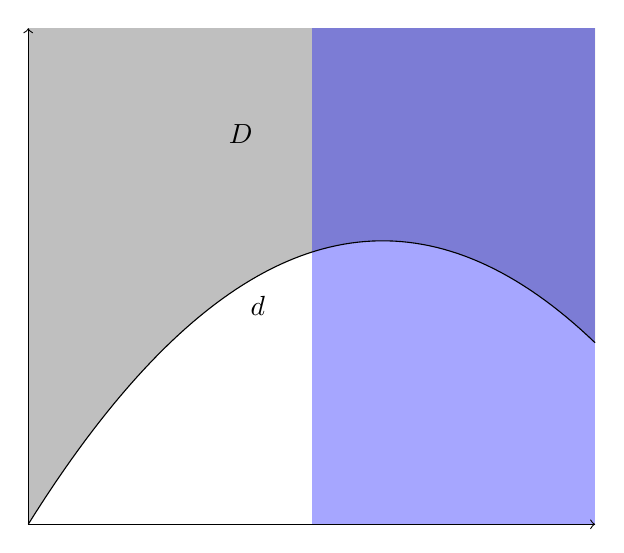
\begin{tikzpicture}[scale=0.9]
		
		% D
		\fill [gray, opacity=0.5, domain=0:8, variable=\x, samples=80]
			(0, 0)
			-- plot ({\x}, {(40/25)*\x + (-4/25)*\x*\x})
			-- ( 8, 7)
			-- ( 0, 7)
			-- ( 0, 0);
		\fill [blue, opacity=0.35] ( 4,0) rectangle ( 8, 7);
		\draw [domain=0:8, variable=\x, samples=80]
			plot ({\x}, {(40/25)*\x + (-4/25)*\x*\x});
		\draw ( 3, 5.5  ) node {$D$};
		\draw ( 3, 3*40/25 - 9*4/25 ) node[anchor=north west] {$d$};

		% axes
		\draw[<-] (0,7) -- (0,0);
		\draw[->] (0,0) -- (8,0);

	\end{tikzpicture}
	\caption{A delegation set $D$ (grey) and the set of allocations that yield agent utility at least $u$ (blue). $1-x(u)$ is the measure of the intersection.}
	\label{fig:AV2010_x}
\end{figure}%
%
In particular, $x(0)$ is the proportion of banned allocations. $x$ is evidently increasing, hence differentiable a.e. with derivative
%
\begin{equation*}
	x' = p f .
\end{equation*}
%
In addition, $x$ must satisfy $\lim_{u \uparrow \infty} x(u) = 1$.


Conditional on there being $N=n$ allocations, then the probability that all allocations that yield at least $u$ are banned is $x(u)^n$. It follows that the (unconditional) probability that all allocations that yield at least $u$ are banned is $\phi(x(u))$, where
%
\begin{equation*}
	\phi(\xi) \coloneqq \sum_{n=0}^\infty \xi^n q(n) .%
		\footnote{$\phi$ is called the \emph{probability generating function (pgf)} of the distribution $q$. Pgfs have certain useful general properties, such as continuity, monotonicity and convexity.}
\end{equation*}


We can now write down the principal's problem formally.
Write $(U,V)$ for an arbitrary random allocation.
For a given boundary $d$, the principal's payoff is
%
\begin{align*}
	\Phi(d)
	&= \int_0^\infty
	\E\left( V \middle| d(u) \leq V \right)
	\dd \phi(x(u))
	\\
	&= \int_0^\infty
	\frac{ \int_{d(u)}^\infty v g(v|u) \dd v }{ p(u) }
	\phi'(x(u)) p(u) f(u) \dd u
	\\
	&= \int_0^\infty V(d,u) \phi'(x(u)) p(u) f(u) \dd u ,
\end{align*}
%
where
%
\begin{equation*}
	V(d,u) 
	\coloneqq \E\left( V \middle| U=u, d(u) \leq V \right) 
	= \frac{1}{p(u)} \int_{d(u)}^\infty v g(v|u) \dd v .
\end{equation*}
%
Her problem is therefore
%
\begin{align*}
	\max_{ d,x,p }
	& \int_0^\infty V(d,u) \phi'(x(u)) p(u) f(u) \dd u
	\\
	\text{s.t.}\quad
	& x' = p f
	\quad \text{a.e.}
	\\
	& \lim_{u \uparrow \infty} x(u) = 1
	\\
	& p(u) = \int_{d(u)}^\infty g(\cdot|u) 
	\quad \text{for every $u \in \R_+$.}
\end{align*}
%
Letting $G(v|u) \coloneqq \int_0^v g(\cdot|u)$, we have
%
\begin{equation*}
	p(u) = 1 - G(d(u)|u) ,
\end{equation*}
%
so that the principal's problem reads
%
\begin{align*}
	\max_{ d, x }
	& \int_0^\infty 
	V(d,u)
	\left[ 1 - G(d(u)|u) \right]
	\phi'(x(u)) f(u)
	\dd u
	\\
	\text{s.t.}\quad
	& x'(u) = \left[ 1 - G(d(u)|u) \right] f(u)
	\quad \text{for a.e. $u \in \R_+$}
	\\
	& \lim_{u \uparrow \infty} x(u) = 1 .
\end{align*}
%
This is an optimal control problem,
with $d$ the control and $x$ the state. The Pontryagin maximum principle gives necessary conditions for optimality. Some conditions on $f$ and $g$ are enough to guarantee that the program is concave, so that the necessary conditions are also sufficient.

One general feature of solutions is that $d(0)=0$ (`no distortion at the bottom'). This is pretty obvious: the only reason to have $d(u) > 0$ is to deter the agent from choosing high-$u$-low-$v$ allocations, but there are no allocations with $u$ lower than zero.

Unsurprisingly, for the special case $q(0)+q(1)=1$ in which the agent never has the choice between multiple allocations,
it is optimal to use the `naïve' delegation policy $d = 0$ (always permit everything).
A few more qualitative things can be said about the solution. When $q$ is the Poisson pmf, a solution is available in closed form.


\paragraph{The literature.}
\textcite{ArmstrongVickers2010} solve for the optimal $d$ using optimal control.
A note: they parametrise their model so that the principal's payoff is $v + \alpha u$ for some $\alpha \geq 0$, so their results are stated somewhat differently.
They derive comparative statics with respect to $\alpha$ (an `ally principle': more aligned preferences lead to more permissive delegation),
consider an extension in which allocations are generated by the agent via costly and unobservable effort (moral hazard),
and show that monetary transfers to the agent may not be used even if available.
They also provide an example of how the principal can do better if the agent is able to propose more than one allocation; this issue is studied further by \textcite{GuoShmaya2022}.



%%%%%%%%%%%%%%%%%%%%%%%%%%%%%%%%%%%
%%%%%%%%%%%%%%%%%%%%%%%%%%%%%%%%%%%
\section{Random mechanisms}
\label{sec:ch4:random}
%%%%%%%%%%%%%%%%%%%%%%%%%%%%%%%%%%%
%%%%%%%%%%%%%%%%%%%%%%%%%%%%%%%%%%%

In the model of the previous section,
suppose that there are two allocations (besides the status quo) for sure (i.e. $q(2)=1$), independently drawn from a binary distribution
that assigns equal probability to $(2,4)$ and to $(3,1)$.
Optimal mechanisms must obviously permit the principal's favourite allocation $(2,4)$;
the only question is whether or not to permit the `tempting' allocation $(3,1)$.
Banning it gives the principal an expected payoff of $\frac{3}{4} \times 4 = 3$,
while allowing it gives her only $\frac{1}{4} \times 4 + \frac{3}{4} \times 1 = 1.75$.
So it is best to ban $(3,1)$ altogether.

But suppose the principal can commit to approve $(3,1)$ with a small but positive probability.
That is, the principal commits to a rule
which specifies for each allocation the probability with which it is approved if proposed.

In particular, suppose she commits to approve $(2,4)$ for sure,
and to approve $(3,1)$ with probability $p \in (0,1)$.
When $(2,4)$ is available, the agent will still prefer to propose it rather than $(3,1)$ provided $2 \geq 3p$, or $p \leq 2/3$.
The random approval mechanism with $p=2/3$ is clearly better:
the principal still gets $4$ whenever $(2,4)$ is available (whether or not $(3,1)$ is available, the agent will propose $(2,4)$),
and additionally, when $(3,1)$ is the only available allocation,
she now earns $1$ with probability $2/3$ rather than zero for sure.

\begin{remark}
	%
	\label{remark:randomisation_commitment}
	%
	If the agent behaves as expected, by proposing $(3,1)$ only when $(2,4)$ is unavailable, then when the principal observes $(3,1)$ being proposed, she will be tempted ex post to approve $(3,1)$ for sure, not just with probability $2/3$.
	When considering random mechanisms,
	we are assuming that the principal can commit ex ante not to give in to such ex-post temptations:
	she is able \emph{credibly} to promise ex ante that she will approve $(3,1)$ with (exactly) probability $p=2/3$.
	That is arguably a very strong assumption. Can you think of situations in which it might be reasonable?
	%
\end{remark}

A taxation principle for random mechanisms lets us restrict attention to `random approval mechanisms', defined by a function $\delta : \R_+^2 \to [0,1]$: the agent proposes an allocation $(u,v) \in \R_+^2$, and it is approved with probability $\delta(u,v)$. (If the proposal is not approved, then the status quo is implemented.)
By analogy with our `upward closed' result, it is easily seen that we may restrict attention to mechanisms $\delta$ such that $\delta(u,\cdot)$ is weakly increasing.

Solving for \emph{optimal} random approval mechanisms appears difficult; no-one has managed it so far, anyway.


\paragraph{The literature.}
\textcite{ArmstrongVickers2010} noted the benefits of randomisation, but did not study random mechanisms systematically.
\textcite{GuoShmaya2022} make progress by replacing our `Bayesian' objective (the principal has some fixed belief about how $A$ is distributed)
with an uncertainty-averse `minmax regret' objective.
This allows them to obtain a clean solution,
and (more importantly?) some nice qualitative insights about how the principal should optimally utilise her power to randomise.



%%%%%%%%%%%%%%%%%%%%%%%%%%%%%%%%%%%
%%%%%%%%%%%%%%%%%%%%%%%%%%%%%%%%%%%
\section{Dynamics}
\label{sec:ch4:dynamics}
%%%%%%%%%%%%%%%%%%%%%%%%%%%%%%%%%%%
%%%%%%%%%%%%%%%%%%%%%%%%%%%%%%%%%%%

There are two dynamic papers in this literature: \textcite{BirdFrug2019,sfb}.



%%%%%%%%%%%%%%%%%%%%%%%%%%%%%%%%%%%
\subsection{IID availability, simple payoffs, budget constraint}
\label{sec:ch4:dynamics:birdfrug}
%%%%%%%%%%%%%%%%%%%%%%%%%%%%%%%%%%%

In \textcite{BirdFrug2019} there is a single allocation $(u,v)$.
The principal prefers this allocation to the status quo,
while the agent does not ($u<0<v$).
We assume that $u+v>0$, so that the allocation $(u,v)$ is (Kaldor--Hicks) efficient.

The principal can `reward' the agent at linear cost to herself;
in other words, she can increase the agent's utility by $r \geq 0$ at a cost of $c r$ to herself, for some fixed $c>0$ that we'll normalise to $c=1$.
A natural interpretation is that $r \geq 0$ reflects a monetary transfer to the agent. (The authors have a more complicated interpretation in terms of randomly-arriving `reward opportunities'.)

The model is dynamic, and the players have the same discount factor $\delta \in (0,1)$. In each period, the allocation $(u,v)$ may or may not be available; the agent knows whether it is, and the principal does not.
Availability is IID over time.
The principal can commit to future rewards (and approval).

As stated, the principal's problem is straightforward:
she can incentivise disclosure by committing to pay the agent $-u$ every time she discloses. Disclosure clearly cannot be incentivised more cheaply, and the principal prefers this mechanism to not incentivising disclosure at all because we assumed that $u+v>0$. So this is what's optimal.

The authors augment this setting with a (per-period) budget constraint for rewards:
the principal only has $b \in (0,-u)$ units of reward resources (e.g. money) in each period. (If we had $b \geq -u$, then the constraint would never bind.)
The authors allow the available resources $b$ to vary randomly between periods;
this doesn't materially affect the results.

The constraint means that with present resources alone,
the agent cannot be rewarded sufficiently to incentivise her to disclose.
So if she is to be incentivised, then she must be promised \emph{future} rewards as well.
This sounds precarious, and it is: if the allocation appears frequently enough, then the principal will eventually be forced to promise to pay the agent $b$ in \emph{every} future period, i.e. to max out her promise-making ability. Once that has happened, the principal cannot incentivise the agent any longer: having pledged all of her future resources, she resigns herself to the status quo allocation being implemented forevermore.

The authors show that this `maxing-out' will happen a.s. in finite time. (If you know some probability theory, then you'll see that this follows from the Borel--Cantelli lemma.)



%%%%%%%%%%%%%%%%%%%%%%%%%%%%%%%%%%%
\subsection{Single breakthrough, general payoffs}
\label{sec:ch4:dynamics:sfb}
%%%%%%%%%%%%%%%%%%%%%%%%%%%%%%%%%%%

In \textcite{sfb}, there is initially available some set $A_0$ of allocations.
At an uncertain time $\tau$, a \emph{breakthrough} occurs, expanding the set of available allocations to $A_1 \supseteq A_0$.
The two sets of allocations are arbitrary, so that payoffs are entirely general.
This allows for any kind of `rewarding the agent' you like, including the linear specification of the previous paper.
No exogenous constraints (e.g. budget) are imposed.
The agent can disclose the availability of the new allocations (i.e. `propose' them) at any time after the breakthrough, but not before.

We characterise optimal mechanisms in this setting. The main finding is that optimal mechanisms have a deadline structure.
